%%%%%%%%%%%%%%%%%%%%%%%%%%%%%%%
% CHAPTER 1: INTRODUCTION
%%%%%%%%%%%%%%%%%%%%%%%%%%%%%%%
%%%%%%%%%%%%%%%%%%%%%%%%%%%%%%%%%%%%%%%%%%%%%%%%%%%%%%%%%%%%%%%%%%%%%%%%%%%%%%%%%%%%%%%%%%
% Richard Boardman PhD Thesis: Improving Tool Support for Personal Information Management
%%%%%%%%%%%%%%%%%%%%%%%%%%%%%%%%%%%%%%%%%%%%%%%%%%%%%%%%%%%%%%%%%%%%%%%%%%%%%%%%%%%%%%%%%%
%%%%%%%%%%%%%%%%%%%%%%%%%%%%%%
% General content meanderings
%%%%%%%%%%%%%%%%%%%%%%%%%%%%%%
% Avoid too much background detail here - move bulk to Literature Review}
% Work towards exploratory thesis, need to focus, structure as a journey
% choice of design-based methodology
% Provide background on research issue, contextualize the thesis, basic scene-setting, orienting commitments, research philosophy.
%%%%%%%%%%%%%%%%%%%%%%%%%%%%%%%%%%%%%%%
% Chopped: relation to HCI discipline
%%%%%%%%%%%%%%%%%%%%%%%%%%%%%%%%%%%%%%%
% This PhD sets out to contribute to the field of Human-Computer Interaction (HCI). . This thesis work has been carried out within the interdisciplinary research field of Human Computer Interaction (HCI). HCI has been defined as the provision of a knowledge base to support the design of \textit{usable} (and useful) computer systems
%%%%%%%%%%%%%%%%%%%%%%%%%%%%%%%%%%%%%%%%%%%%%%%%
% Intro
%%%%%%%%%%%%%%%%%%%%%%%%%%%%%%%%%%%%%%%%%%%%%%%%
% 1. What is PIM
% 2. PIM problems
% 3. Focus: PIM integration
%		 focus on storage/org within PIM and or unification??? NO
% 4. Establish rationale/motivation:
% 		Who will benefit?
%			Why is it important?
% 		Why is it worthwhile?
%			under-researched etc.
%			critical activity - knock-on benefits
% 5. Why I was compelled to work in this area
%			Driving interest
% 6. State core thesis/claim
%%%%%%%%%%%%%%%%%%%%%%%%%%%%%%%%%%%%%%%%%%%%%%%%
% Personal information management (PIM) is introduced as the research area for the thesis.
% avoid too much detail here - shift most to Conceptual Framework and  Literature Review}
% Concrete examples (both physical and digital) - illustrate research area
%%%%%%%%%%%%%%%%%%%%%%%%%%%%%%%%%%%%%%%%%%%%%%%%

%%%%%%%%%%%%%%
% TO PLACE
%%%%%%%%%%%%%%
%%%%%%%%%%%%%%%%%%%%%%%%%%%%%%%%%%
% Brief summary of current tools
%%%%%%%%%%%%%%%%%%%%%%%%%%%%%%%%%%
% Brief survey of current tools
% Many software tools allow users to manage personal information. Today's computing environments contain a wide range of software tools that allow an individual to manage information in a range of technological formats (e.g. email messages, web bookmarks, files, calendar entries, contacts). 
% General trend: More space -- more items -- more organizing/tidying to do (in the old days people might be more careful about what they acquire and keeping it tidy would therefore be easier). Paradox - more items, more folders, more organizing to do

%%%%%%%%%%%%%%%%%%%%
% General context
% NB: PIM not specific to computers
% Very brief definition - do not need too much detail
% 	Do not get drawn into a discussion here, leave that for Chapter 2
% 	Also concisely define `personal information' NB: Jens: what is limit? Excel cells?
% PIM has been defined in terms of four related activities performed by an individual: the \textit{acquisition} of information, the \textit{organization} of those items, the \textit{maintenance} of the collections of information so formed, and the subsequent \textit{retrieval} of information for reuse~\citep{barreau:95}.
%%%%%%%%%%%%%%%%%%%%
% Today's computing environments contain a wide range of software applications that allow the management of different forms of digital information.
% A prime characteristic of human nature is to acquire and keep items of value.  In both the physical and digital domains, our personal environments become populated with the items we accumulate as our lives unfold.
Personal Information Management (PIM) is an umbrella term used to describe the collection, storage, organization and retrieval of items of digital information (e.g. email, files, appointments, reminders, contacts, bookmarks) by an individual in their personal computing environment~\citep{ml:88}.  \citet{Bergman:03} compare PIM with ``general information management'' in which a professional -- such as a librarian -- manages information for other people. In contrast, with PIM the onus is on an individual to manage his/her own information.  PIM is a fundamental aspect of everyday computer-based activity in both work and home contexts~\citep{bn:95}, performed by \textit{``millions of users many times a day''}~\citep{Whittaker-rta:00}.

%%%%%%%%%%%%%%%%%%%%%%%%%%%%%%%%%%%%%%%%%%%%%%%%%%%%%%%%%%%%%%%%%%%%%%%%%%%%%%%%%%%%%
%%%%%%%%%%%%%%%%%%%%%%%%%%%%%%%%%%%%%%%%%%%%%%%%%%%%%%%%%%%%%%%%%%%%%%%%%%%%%%%%%%%%%
% \section{The Struggle for Control of the Workspace}
% \label{intro:user-problem}
%%%%%%%%%%%%%%%%%%%%%%%%%%%%%%%%%%%%%%%%%%%%%%%%%%%%%%%%%%%%%%%%%%%%%%%%%%%%%%%%%%%%%
% In this section the problems encountered by computer users are described.
%%%%%%%%%%%%%%%%%%%%%%%%%%%%%%%%%%%%%%%%%%%%%%%%%%%%%%%%%%%%%%%%%%%%%%%%%%%%%%%%%%%%%
%%%%%%%%%%%%%%%%
% User Problems
%%%%%%%%%%%%%%%%
% compelling user problems, there is a need for research)
%	Evidence (anecdotal and solid research findings) of user struggles in PIM. Time spent.
%	Some have framed the problem in terms of being too easy to acquire, too hard to organize and find
% Implications of this -- overheads (impact on productivity?/futzing) and satisfaction. Has computer lived up to its promise as a time-saving device?
% Real problem, worth-while issues/phenomena to investigate  but lots of challenges! Complex/open-ended problem space
%%%%%%%%%%%%%%%%%%%%%%%%%%%%%%%%%%%%%%%%%%%%%%%%%%%%%%%%%%%%%%%%%%%
% Towards narrower/focused scope of problems *(no - do this later)
%%%%%%%%%%%%%%%%%%%%%%%%%%%%%%%%%%%%%%%%%%%%%%%%%%%%%%%%%%%%%%%%%%%
% Focus on Org/storage}: Anxiety of order (Bacon, Dewey -- craving for order obsessive/compulsive, Levy p129), have to organize the organizing.
% Cross-tool problems
% Problems in particular tools
% Limitations (e.g. limits of hierarchy, again with evidence)
% %%%%%%%%%%%%%%%%%%%%%%%%%%%%%%%%%%%%%%%%%%%%%%%%%%%%%%%%%%%%%%%%%%%%%%%%%%%%
%%%%%%%%%%%%%%%%%%%%%%%%
% Users have problems
%%%%%%%%%%%%%%%%%%%%%%%%
% However, there is much (ANECDOTAL) evidence that PIM 
% Studies of PIM have highlighted the problems users encounter
% have shown that many computer users encounter a wide range of problems using current PIM-tools
% and the limitations of the organizational support offered by tools, typically based on the traditional hierarchy (Lansdale, 1988). 
% However, there is much evidence that current tool support for PIM is unsatisfactory, and many users encounter difficulties in managing information~\citep{ml:88,bn:95}.
Like managing one's possessions in the physical world, studies have reported that PIM is frequently a chore~\citep{tm:83,ml:88,bn:95,Whittaker-email:96,kftf:01}.
These studies indicate that PIM is poorly supported by current technology, and that many users struggle to handle, classify and retrieve the information that they accumulate over time in tools such as the file system, the desktop and email. There is widespread concern that problems with PIM impact work productivity~\citep{ml:88,sellen:01,Jones:04} and user experience~\citep{Bellotti:00}.
%%%%%%%%%%%%%%%%%%%%%%%%%%%%%%%%%%%
% TRENDS: problems getting worse!
%%%%%%%%%%%%%%%%%%%%%%%%%%%%%%%%%%%
% It is suggested that this is an increasingly important user problem. (relevance/number of users/ferocity/trends)
% * Information overload (quantity and variety).  Access to more info, the web as \textit{aleph} (Levy).
% Number of tools~\citep{web-sjohnson:02}
% More storage potential, too easy to acquire, keep more, retrieval is the key problem!
% Tool complexity (but cf. Apple iApps)
Several current trends are exacerbating these problems.  Firstly, computer users are being exposed to more and more information~\citep{sellen:01}, much of it personally managed.  This is partially due to the success of email and the web in transferring previously ``real-world'' activities to the digital domain.  Secondly, increased storage capacity on interactive devices means that users are able to collect more information~\citep{bell:02}, leading to more management overheads.  Thirdly, users are managing information in more technological formats in more software applications~\citep{Bellotti:00,Kaptelinin:03}.
Finally, many users are managing information in more places -- for example on multiple desktop computers, laptops and on PDA devices and mobile phones.

%%%%%%%%%%%%%%%%%%%%%%%%%%%%%%%%%%%%%%%%%%
% DESIGN CHALLENGE
% PIM as a design priority
% Bottom line: little change for users
%%%%%%%%%%%%%%%%%%%%%%%%%%%%%%%%%%%%%%%%%%
Improving the design of PIM tools is therefore a compelling challenge for interface developers.  Since this is an area in which millions of people encounter everyday problems, there is a huge potential market for improved PIM tools.  However, it should be noted that this challenge is not new and many of the problems encountered by users today were observed more than a decade ago, e.g.~\citep{tm:83,ml:88}.  This is not surprising as \citet{Cooper:03} observes that the designs in common usage have changed little over the two decades since the invention of the folder hierarchy and the Desktop metaphor in the 1960s and 1970s\footnote{See \textbf{Section~\ref{bg:pim-history}} for further discussion on the roots of PIM technology.}.  Although many new designs have been proposed, few have been successful.   However, much design effort, in both the commercial and open-source sectors, continues to be aimed in this direction, and a number of major software companies consider improving PIM support to be a key objective, e.g. Microsoft~\citep{Gates:03}. There is a general acceptance that new tools are needed, but no consensus as to route for design.




%(e.g. Microsoft citep Gates speech, Apple citep Jobs speech). 
%%%%%%%%%%%%%%%%%%%%%
% But changed little
%%%%%%%%%%%%%%%%%%%%%
% Many ideas around - but overall, there's been little change! 

%%%%%%%%%%%%%%%%%%%%%%%%%%%%%%%%%%%%%%%%%%
% VERY HIGH-LEVEL SUMMARY OF THE THESIS
% Core research hypothesis?
% In this thesis it is argued
% This thesis sets out to 
% (treated?) considers?
% My particular stance!
% The Rick view
%%%%%%%%%%%%%%%%%%%%%%%%%%%%%%%%%%%%%%%%%%
% PIM in general
% %%%%%%%%%%%%%%
% % In particular, this thesis work is aimed at improving the usability of a particular class of computer systems - those that support Personal Information Management (PIM) -- one particular application domain of computing technology.
% %%%%%%%%%%%%%%%%%%%%%%%%%%%%%%%%%%%%%%%%
% % main claim: PIM as a CT activity
% %%%%%%%%%%%%%%%%%%%%%%%%%%%%%%%%%% 
% move away from independent PIM systems
% takes the view that PIM support should be improved from a cross-tool perspective.
% Not limited to particular applications.
% to guide designers in providing integration between PIM-tools.
% THINK: where to define cross-tool?
% My holistic view -- state cross-tool perspective and its justification.
% Take a step-back from application-centric view. Similar views.
% explore potential to unify PIM. Integration}
% Provide more coherent support across workspace as a whole
% and thus deal with distribution across multiple tools
%%%%%%%%%%%%%%%%%%%%%%%%%%%%
% Sum up method here?
% e.g. production of artifact
The high level aim of this doctoral research is to improve HCI knowledge regarding PIM, and thus provide guidance for the designers of PIM-tools.  In particular, the thesis focus is on investigating the potential to improve integration between PIM-tools.
%%%%%%%%%%%%%%%%%%%%%%%%%%%%%%%%
% In particular: INTEGRATION
% include quotes from Gates
%%%%%%%%%%%%%%%%%%%%%%%%%%%%%%%%
%%%%%%%%%%%%%%%%%%%%%%%%%%
% Focus on integration/unification
% integration: to what end?
%%%%%%%%%%%%%%%%%%%%%%%%%%
% Basic taxonomy of solutions/design strategies. Consider intra-tool and unification.    
% In the research domain, many systems have been proposed to improve support for PIM.  
% There is certainly a high level of interest in PIM-integration within the design community, as a means of improving support for users. % As well as design directed at improving specific PIM tools such as email (e.g. ~\citep{mailcat:99})
% here has been extensive interest in the potential to improve integration between tools.  This design strategy for improving PIM support, that of providing integration between PIM tools, is the focus of this thesis. Examples of commercial systems that have offered enhanced integration to date include BeOS~\citep{Giampaolo:98,Scopeware}, Scopeware~\citep{} and SixDegrees~\citep{SixDegrees}. 
Researchers have highlighted the particular problems caused by the the fragmentation of an individual's information across a range of distinct tools such as files and email~\citep{Bellotti:00,Kaptelinin:03}.  Therefore, there is ongoing design effort in developing more integrated PIM technology. Many novel technologies have been proposed in both the commercial~\citep{Giampaolo:98}, open-source~\citep{Chandler:03}, and research domains~\citep{dourish:99a,Bellotti:03,Kaptelinin:03}.  Furthermore, at the time of writing, the two major commercial personal operating system vendors, Microsoft and Apple, are planning enhanced PIM integration in the next versions of their operating systems~\citep{Fried:04}. % MS-Windows~\citep{winfs:03}, and MacOS respectively. % citep Apple? 
% Also a number of open-source systems are aimed at providing increased integration between tools, e.g. OSAF-Chandler~\citep{}. % GNOME Storage~\citep{} 

% In particular this research considers PIM as a \textit{cross-tool} activity -- one distributed across multiple tools, and investigates the potential to improve integration between PIM-tools. The term \textit{cross-tool} is proposed to describe technology that provides integration between PIM-tools.

%%%%%%%%%%%%%%%%%%%%%%
% Chapter overview
%%%%%%%%%%%%%%%%%%%%%%
% Chapter 1 presents a brief overview of the research area: personal information management, the research problem within this area, and aims/objectives and choice of method for the thesis. 
% two sections summarize the problem space addressed by the thesis from two perspectives: (a) that of the real-world problems encountered by users in managing information (\textbf{Section~\ref{intro:user-problem}}), and (b) that of the limitations of prior research (). % i.e. results of lit review
The rest of this chapter is structured as follows.  Firstly, \textbf{Section~\ref{intro:research-problem}} highlights a number of limitations of previous research on PIM, taking a particular focus on that related to improving integration between PIM-tools.  Based on these limitations, \textbf{Section~\ref{intro:aims}} states the research objectives of the thesis, and  \textbf{Section~\ref{intro:approach}} details the design-based research methodology employed.  Finally, \textbf{Section~\ref{intro:thesis-overview}}, presents an outline of subsequent chapters, and details the contributions offered in the thesis. 

%%%%%%%%%%%%%%%%%%%%%%%%%%%%%
% Link to the next section
%%%%%%%%%%%%%%%%%%%%%%%%%%%%%
% The next section, surveys related HCI research to date.
% \textbf{Section~\ref{intro:research-problem}} provides a high-level survey of research to date.
% In parallel to activity in the design domain, there has been much related HCI research, as discussed in the next section.



















%%%%%%%%%%%%%%%%%%%%%%%%%%%%%%%%%%%%%%%%%%%%%%%%%%%%%%%%%%%%%%%%%%%%%
%%%%%%%%%%%%%%%%%%%%%%%%%%%%%%%%%%%%%%%%%%%%%%%%%%%%%%%%%%%%%%%%%%%%%
\section{HCI Research on PIM}
\label{intro:research-problem}
%%%%%%%%%%%%%%%%%%%%%%%%%%%%%%%%%%%%%%%%%%%%%%%%%%%%%%%%%%%%%%%%%%%%%
%%%%%%%%%%%%%%%%%%%%%%%%%%%%%%%%%%%%%%%%%%%%%%%%%%%%%%%%%%%%%%%%%%%%%
%%%%%%%%%%%%%%%%%%%%%%%%%%%%%%%%%%%%%
% Under-researched - need for more
%%%%%%%%%%%%%%%%%%%%%%%%%%%%%%%%%%%%%
%  Finally, state conclusion of literature review, PIM is under-researched (research problems/gaps)
% Problem2: state of research
% Practice >> Research
% NB: don't discuss reasons why here, leave that until the discussion
% This should be a sneak preview of the conc of the Lit Review
% The overall state of HCI knowledge relating to PIM is summarized. 
% THINK: STRUCTURE - first PIM in general, secondly PIM-integration/cross-tool:
%%%%%%%%%%%%%%%%%%%%%%%%%%%%%%%%%%%%%%
% IN GENERAL - WHAT CAN HCI RESEARCH OFFER?
%%%%%%%%%%%%%%%%%%%%%%%%%%%%%%%%%%%%%%
% HCI research offers guidance for the designers of tools, by providing better understanding of user needs, through design methods and through the evaluation of trial interfaces (citep).
% A primary objective of HCI research is to provide a knowledge base to support the design of usable interactive artefacts~\citep{Sutcliffe:00}. In this section, HCI research on PIM is discussed.  It is argued that despite the importance of PIM, it has been significantly under-researched. In particular there is a lack of HCI knowledge to provide guidance for the design of PIM-integration technology.
%%%%%%%%%%%%%%%%%%%%%%%%%%%%%%%%%%%
% Two main areas of research: (1) studies and (2) design
%%%%%%%%%%%%%%%%%%%%%%%%%%%%%%%%%%%
The literature review in \textbf{Chapter~\ref{chapter:review}} identifies two main areas of PIM-related research: (a) empirical studies of user behaviour, and (b) explorative design and prototyping.  A brief overview is provided of previous research as follows.
% Each is now considered in terms of the support the respective body of knowledge can offer the designers of PIM-integration technology.

%%%%%%%%%%%%%
% Studies
%%%%%%%%%%%%%
%%%%%%%%%%%%%%%%%%%%%%%%%%%%%%%%%%%%%%%%%
% Whittaker: lack of research to date
%%%%%%%%%%%%%%%%%%%%%%%%%%%%%%%%%%%%%%%%%
% % However Whittaker et al. [17] note the relative lack of empirical research on an activity ``carried out by millions of users, multiple times a day''. 
% Whittaker et al. (2000) ref  highlight the general lack of progress within HCI towards understanding PIM.  
% Relative lack of attention within HCI (contrast with information-seeking, CSCW). Lack of systematic research/robust body of knowledge and in-depth investigation (emphasise despite evidence that this is a fundamental everyday computer-based activity, core task)~\citep{Whittaker-rta:00}
% There is consequently a lack of systematic research knowledge to guide the design of PIM-tools.  In particular Whittaker \textit{et al}. highlight the need for improved  % terminological muddle
% In addition, little theoretical work has been carried out in the area.  There is a lack of appropriate theoretical apparatus, e.g. descriptive vocabulary for talking about PIM-integration.
%%%%%%%%%%%%%%%%%%%%%%%%%%%
% Why is PIM so ignored?
%%%%%%%%%%%%%%%%%%%%%%%%%%%
% This is a compelling real-world user problem, and one that leads to the question why HCI has devoted so scant attention to it? Under-researched. Influenced our choice of methodology. We uncover possible reasons for this lack of attention/many challenges involved in researching this area. 
As discussed above, a number of studies have investigated PIM behaviour. These have offered many pertinent observations of user strategies and needs, and provided many design recommendations.  However, \citet{Whittaker-rta:00} claim that PIM has been relatively under-researched despite this existing body of work. They argue that considering the fundamental nature of PIM, a handful of studies does not constitute a body of systematic research. In particular, they highlight the need for consistent descriptive vocabulary, theoretical models and evaluation metrics.

%%%%%%%%%%%%%%%%%%%%%%%%%%%%%%%%%%%%%%%%
% Focused on particular applications
%%%%%%%%%%%%%%%%%%%%%%%%%%%%%%%%%%%%%%%%
% Add a couple of examples. Several have called for improved integration (citep)
% It is argued that cross-tool empirical data is required to provide increased understanding of PIM from a cross-tool perspective, and thus in turn provide a firmer foundation for cross-tool design (i.e. integration). General application-centricity, inherently piecemeal
% There is especially little HCI knowledge relating to improving integration between PIM-tools.
% Although many studies observing problems (although application-centric), there is a lack of understanding of what users are doing and what they need. 
% Secondly, little attention has been paid to how PIM strategies change over time. One exception is B�lter [2] who proposed a model of strategy changes in email (see Figure 1). 
% One final limitation, identified in \textbf{Chapter~\ref{chapter:review}} is an over-focus on technical/professional users.
In this thesis, it is emphasised that particularly little research attention has been directed to the question of PIM integration. \textbf{Chapter~\ref{chapter:review}} notes how most empirical studies have focused on specific tool contexts, such as email.  Although it has been observed that people often employ multiple PIM tools in support of their high-level activities~\citep{Kaptelinin:96}, there has been little investigation of PIM as a cross-tool activity.  Do individuals employ similar strategies in email as in files? How are PIM tools used together?  Such questions must be addressed to provide a firm empirical foundation for design work aimed at improving PIM-tool integration.

%%%%%%%%%%%%
% Design
%%%%%%%%%%%
The second area of research has focused on the exploratory prototyping of new PIM interfaces.  As in the commercial domain, there has been extensive interest in the potential to improve integration between tools. Two main approaches can be identified in efforts to improve integration: (a) \textit{embedding} support for managing multiple types of information within an existing tool. e.g.~\citep{Bellotti:03} and (b) \textit{unifying} interaction with multiple types of information (e.g. files and email) within a consolidated interface. Examples of this second genre include \textit{Stuff-I've-Seen}~\citep{Dumais:03a} which provides a unified search interface, and \textit{UMEA}~\citep{Kaptelinin:03} which enables the organization of multiple types of information in terms of projects.  The term \textit{cross-tool} is proposed to describe design that provides integration between PIM-tools.
% Numerous research have been proposed that offer innovative integration mechanisms. 
This body of cross-tool design research can be criticised for not making an effective contribution to HCI knowledge, for two key reasons:
\begin{enumerate}
% Be careful: ContactMap is founded on empirical data
\item Firstly, much of this cross-tool design work has been driven by technological innovation rather than founded on empirical user requirements. As noted above, empirical work to date has focused on the management of particular types of information within specific PIM tools (e.g. email).  % As noted above, little knowledge exists concerning the needs of users beyond the boundaries of specific PIM tools. % As noted above, there is a need for cross-tool empirical data to provide a foundation for such cross-tool design.
% Although many innovative designs have been proposed, a mismatch can be highlighted between the tool-specific studies that have provided observations about users' activities and problems -- and the substantial design effort directed at cross-tool integration. 

\item Furthermore, most cross-tool systems have not been evaluated.  Although, many systems have been highly innovative and offered much in the way of new technology, such ``radical invention''~\citep{Whittaker-rta:00} can raise significant usability issues. This means that evaluation is particularly important to confirm the benefits claimed by designers. One factor which may contribute to the infrequency of evaluation, is the lack of agreed metrics for comparing different PIM designs~\citep{Whittaker-rta:00}. % 	little methodological guidance concerning the evaluation of PIM tools. Lack of appropriate methods attuned to the nature of PIM. Hint at similar problems with other activities

%	\item Thirdly, proposed technologies have been ``revolutionary''. This may be a key reason why they have not been taken up. It is also means that they are hard to evaluate. % Here it is argued that a primary reason for the lack of evaluation is the ambitious, revolutionary nature of the designs proposed. 

\end{enumerate}

The next section reports the specific objectives of this research.


%\newpage
%%%%%%%%%%%%%%%%%%%%%%%%%%%%%%%%%%%%%
%%%%%%%%%%%%%%%%%%%%%%%%%%%%%%%%%%%%
\section{Research Agenda}
\label{intro:aims}
%%%%%%%%%%%%%%%%%%%%%%%%%%%%%%%%%%%%
%%%%%%%%%%%%%%%%%%%%%%%%%%%%%%%%%%%%%
%%%%%%%%%%%%%%%%%%%%%%%%%%%%%%%%%%%%%%%%%%%%%%%%%%%%%%%%%%%%%%%%%%%%%%%%%%%%%%%
% RESEARCH PROBLEM/QUESTION
% THINK: can I merge Problemi 1 and 2 to form a cohesive research statement?
% THINK: can I coalesce needs in a single method justification?
% Can I relate the research problem in the wider context?
%%%%%%%%%%%%%%%%%%%%%%%%%%%%%%%%%%%%%%%%%%%%%%%%%%%%%%%%%%%%%%%%%%%%%%%%%%%%%%%
%%%%%%%%%%%%%%%%%%%%%%%%%%%%%%%%%%%%%%%%%%%%%%%%%%%%%%%%%%%%%%%%%%%%%%%%%
% RESEARCH PHILOSOPHY
% THINK: define research philosophy and position within literature space. This should lead onto choice of research paradigm and methods}
%%%%%%%%%%%%%%%%%%%%%%%%%%%%%%%%%%%%%%%%%%%%%%%%%%%%%%%%%%%%%%%%%%%%%%%%%
%%%%%%%%%%%%%%%%%%%%%%%%%%%%%%%%%%%%%%%
% Huge area - therefore need to focus
% Therefore exploratory nature
%%%%%%%%%%%%%%%%%%%%%%%%%%%%%%%%%%%%%%%
% Aims, goals
% Could also be termed `Research questions' (Weiss-Lijn)
% What am I going to do to solve the problem
% Need to match objectives with goals later!
%%%%%%%%%%%%%%%%%%%%%%%%%%%%%%%%%%%%%%
% Expand on interest in PIM-integration/unification as a design strategy.
% Thesis as investigation of its potential.}
% THINK: Focus on organization/anxiety-of-order???}
%%%%%%%%%%%%%%%%%%%%%%%%%%%%%%%%%%%%%%
%%%%%%%%%%%%%%%%%%%%%%
% DRIVING INTERESTS/orienting commitments - merged into objectives
% * Desire to create an artefact, based in empirical data, and evaluated. Good HCI practice. Holistic package - complete the cycle of study, design and evaluation (describe in terms of task-artifact cycle). Practical -- applicable work. 
% * Belief in compelling problem space - user burden, can I help?
% * ready to explore
%%%%%%%%%%%%%%%%%%%%%%%%%%%%%%%%%%%%%%%%%%%%%%%%%%%%%%%%%%%%%%%%%%%%%%%%%%%%%%%
% FROM OLD CHAPTER 4: \textbf{Section~\ref{review:research-agenda}} presents a research agenda that sets out the initial exploratory route taken in this body of research.  The agenda is updated after the exploratory study work presented in \textbf{Chapter 4}.
%%%%%%%%%%%%%%%%%%%%%%%%%%%%%%%%%%%%%%%%%%%
% STATEMENT OF PROBLEM BEING ATTACKED
% DIMENSION 1: the user problem
% DIMENSION 2: the research problem
%%%%%%%%%%%%%%%%%%%%%%%%%%%%%%%%%%%%%%%%%%%
% DIANE: why is this a HCI problem?
%			need to aid designers
%%%%%%%%%%%%%%%%%%%%%%%%%%%%%%%%%%%%%%%%%%%
%%%%%%%%%%%%%%%%%%%%%%%%%%%%%%%%%%%%%%%%%%%
% DISCUSSION: Anti turn towards the social
%%%%%%%%%%%%%%%%%%%%%%%%%%%%%%%%%%%%%%%%%%%%
% \textit{NB: Turn towards social has two aspects: (1) groups, (2) non-lab. My work fits in with second but not first. Another trend is an emphasis on new technologies}
% expand to groups, non-lab, new technologies} (Dourish, Rogers, IDB, Carroll97).
% albeit paying attention to the social context in which their computer usage is set). 
% * As such it contrasts with the recent research climate in HCI.
% * also mention focus on revolutionary design?
%%%%%%%%%%%%%%%%%%%%%%%%%%%%%%%%%%%%%%%%%%%%
% Speculation about new paradigms for education, work, and leisure activity have become rampant in the field and in the culture at large.
Much has been written on HCI's recent ``turn towards the social'', e.g. 
\textit{``The portrait of a solitary user finding and creating information in a computer became background to the portrait of several people working together at a variety of times and places''}~\citep{Carroll-review:97}.  Although the recent trend \textit{towards the social} has opened up many interesting areas for research, it has also contributed towards many core everyday computer-based activities such as PIM being under-researched~\citep{Whittaker-rta:00}.  Turning the pages of recent HCI conferences reveals a wealth of research directed at collaborative and social interfaces, but very little on important everyday activities such as PIM.  This thesis seeks to help redress this balance by taking a conscious turn back in the other direction, away from collaborative activities back towards the individual user and a focus on the most personal of activities, PIM.  
% careful PIM: has collaborative aspects


%%%%%%%%%%%%%%%%%%%%%%%%
% ORIENTING INTERESTS
%%%%%%%%%%%%%%%%%%%%%%%%
% The author's initial interests which he brought to the research are described before the initial research objectives are presented.
%%%%%%%%%%%%%%%%%%%%%%%%
% Interest in DESIGN
%  As well as the general interest in integration, another key interest of the author was in design -- in actually implementing the fruits of his research in a concrete artefact which could then be evaluated. 
%% Need to pursue integration-design in an incremental manner, need for requirements, 
%% Balance what I want to do with what is pragmatically possible (what I'm best-equipped to do)

%% NEWPAGE HACK
\newpage
%%%%%%%%%%%%%%%%%%%%%%%%%%%%%%%%%%
\subsection{Objectives}
%%%%%%%%%%%%%%%%%%%%%%%%%%%%%%%%%%

%%%%%%%%%%%%%%%%%%%%%%%%%%%%
% AIMS/GOALS/OBJECTIVES
%%%%%%%%%%%%%%%%%%%%%%%%%%%%
% Guided by the interests described above, and building on the limitations of previous work in the area of improving integration -- the research was inherently cross-tool: i.e. not focused on a specific application.
% The thesis objectives are defined as follows: (1) to build on current understanding, (2) to provide guidance for designers.
The thesis objectives are outlined as follows:
\begin{enumerate}

%%%%%%%%%%%%%%%%%%%%%%%%%%%%%%%%%%%%%%%%%%%%%%%%%%%%%%%%%%%%%%%%%%
% EMPIRICAL : Objective 1: To build on current understanding}
%%%%%%%%%%%%%%%%%%%%%%%%%%%%%%%%%%%%%%%%%%%%%%%%%%%%%%%%%%%%%%%%%%
% Requirements for design.
% provide evidence/description
% Under-researched. Accept observations of relative lack of attention that PIM has received to date within HCI and take steps towards alleviating it. Need for more understanding of core phenomena. Emphasise grounding in empirical data. Empirical stance adopted
% % There is a lack of understanding of fundamental everyday computer-based activities  such as PIM. Importance of grounding in user experiences with the current generation of PIM artefacts (concern for ecological validity).  Understand the world. Study real practice. Use to develop understanding of PIM. 
%%%%%%%%%%%%%%%%%%%%%%%%%%%%%%%%%%%%%%%%%%%%%%%%%%%%
% The first objective was to provide improved understanding of personal information management, with a particular focus on investigating user needs and issues relating to integration between PIM-tools.
%%%%%%%%%%%%%%%%%%%%%%%%%%%%%%%%%%%%%%%%%%%%%%%%%%%%
%%%%%%%%%%%%%%%%%%%%%%%%%%
% ENVISAGED CONTRIBUTION
% The planned method to achieve this objective was to carry out a cross-tool study. The study would provide increased cross-tool understanding of PIM, and so provide an empirical foundation for cross-tool design work aimed at improving PIM integration.
%%%%%%%%%%%%%%%%%%%%%%%%%%%%%%%%%%%%%%%%%%%%%%%%%%%%
\item \textit{To develop increased understanding of PIM practices and related user problems} -- In particular, the researcher set out to investigate user needs and issues relating to PIM integration, and thus provide a firm empirical foundation for design work in this area. 
%%%%%%%%%%%%%%%%%%%%%%
% LEAD -> THEORETICAL
%%%%%%%%%%%%%%%%%%%%%%%
A secondary aim was to develop theoretical models to describe and explain empirical observations.


%%%%%%%%%%%%%%%%%%%%%%%%%%%%%%%%%%%%%%%%%%%%%%%%%%%%%%%%%%%%%%%%%%%%%%%%%%
% DESIGN/EVALUATION : Objective 2: To provide guidance for designers}
%%%%%%%%%%%%%%%%%%%%%%%%%%%%%%%%%%%%%%%%%%%%%%%%%%%%%%%%%%%%%%%%%%%%%%%%%%%%%
% improved tool support for PIM.
% \textit{The author embarked on the work with a strong interest in design, and a background in engineering, which lead to the intention to create an interactive artefact. Commitment to simplifying?  Interest in non-professional/non-technical users?~\citep{web-good-easy:01}}
% Propose technology and evaluate, contrast with more ambitious programs to revolutionize the desktop.
% To design and evaluate new PIM technology in practice (real users, real data, real tools, real environment, over time). Artefact generation. Yet need to do so systematically and contribute to HCI knowledge-base.
%%%%%%%%%%%%%%%%%%%%%%%%%%%%%%%%%%%%%%%%%%%%%%%%%%%
% THE OBJECTIVE
% The second objective was to produce a set of design recommendations regarding the design of improved PIM tools, particularly design work aimed at improving PIM integration.
% This objective was to be achieved through design/evaluation experience.
% The intention was to use findings from the initial study to form grounded design rationale to direct the design.
%%%%%%%%%%%%%%%%%%%%%%%%%%%%%%%%%%%%%%%%%%%%%%%%%%%
% THE METHOD
%%%%%%%%%%%%%
% Due to the lack of appropriate methodology, a parallel aim was to explore issues related to the evaluation of PIM tools, particularly those aimed at improving PIM integration. 
%%%%%%%%%%%%%%%%%%%%%%%%%%%%%%%%%%%%%%%%%%%%%%%%%%%
\item \textit{To propose, implement and evaluate an empirically-grounded means of PIM-integration mechanism} -- The author embarked upon the research programme from a background in computer science, and had a keen interest in developing a new form of PIM-integration.  A key interest was to improve upon the limitations of previous prototyping in the area by emphasising empirical grounding and evaluation.
% However, in contrast to most previous design work in the area, the intention was t


 
 %%%%%%%%%%%%%%%%%
% METHODOLOGICAL
%%%%%%%%%%%%%%%%%
% Methodological: Explore potential of cross-tool approach for both researchers and designers of cross-tool approach. Evaluation: explore ways of doing effective evaluation.  To explore issues related to the evaluation of PIM designs, particularly those directed at improving PIM integration.
% regarding appropriate methodology
% devise appropriate methodology to support the above objectives of investigating PIM, and designing and evaluating PIM-integration mechanisms.  Furthermore, based on these experiences, to produce a set of recommendations regarding the design of PIM interfaces, particularly those aimed at improving PIM integration.
\item \textit{To devise methodological recommendations for future research and design work in the area of PIM-integration} -- The final objective was to provide methodological guidance for future work, derived from the experience of pursuing this course of research.  In particular, \citet{Whittaker-rta:00} note the need for the identification of evaluation metrics.

\end{enumerate}

The next section discusses the methodological approach employed in the thesis to achieve the above objectives.

%%%%%%%%%%%%%%%%%%%%%%%%%%%%%
\subsection{Approach}
%%%%%%%%%%%%%%%%%%%%%%%%%%%%%%%%%%
\label{intro:approach}
%%%%%%%%%%%%%%%%%%%%%%%%%%%%%
% Need justification; based on research principles and pragmatic considerations
% Take inspiration from other researchers and my own orienting commitments
% Total/partial adherence to method X (have weasel?)
% Strong empirical stance
% Systematic/applied
% Exploratory -> Focused
%%%%%%%%%%%%%%%%%%%%%%%%%%%%%
% SP: See Chapter 2 for more information on research paradigm
%%%%%%%%%%%%%%%%%%%%%%%%%%%%%
%	Attempt to bridge three contexts: the user, the researcher and the designer.
% Foot in three camps.  Me as user (pre-conceptions). 
%		\item User -- empirical study and my experience
%		\item Researcher -- understand the world, requirements gathering, analysis
%		\item Designer -- change the world
% Employ Task-artefact cycle as theoretical/methodological perspective towards the work
%%%%%%%%%%%%%%%%%%%%%%%%%%%%%

%%%%%%%%%%%%%%%%%%%%%%%%%%%%%%%%%%
%\subsubsection{Selection of Research Methods}
%%%%%%%%%%%%%%%%%%%%%%%%%%%%%%%%%%
% This section presents the selected research methodology and justifies its selection.

%%%%%%%%%%%%%%%%%%%%%%%%%
% Classic HCI dilemma
%%%%%%%%%%%%%%%%%%%%%%%%%
The selection of appropriate research methodology is a common HCI dilemma.  As an interdisciplinary research field, HCI offers many competing research paradigms and methodologies, each with own way of contributing to the HCI knowledge base~\citep{Sasse:97}.
%%%%%%%%%%%%%%%%%%%%%%%%%%%%%%%%%%%%%%%%%%%%%%%%%%
% Selection of design-centered methodology
%%%%%%%%%%%%%%%%%%%%%%%%%%%%%%%%%%%%%%%%%%%%%%%%%%
% , chosen as it matches the two \textbf{orienting commitments} of this research:
% Blomberg et al.~\citep{blomberg:96} similarly advocate a design-centred approach through two complementary commitments design and research to support each other and improve~\citep{blomberg:96}.
% Design-based research is selected as an appropriate methodology to enable the candidate to experience design issues at first hand. Turn towards design science route. Promise of design-based research methodology. Subscribe to design-based research methodology. Outline how to do research by this approach. Outline how to add to HCI KB according to~\citep{jc:00}. Recap pros and cons and how I will account for them.
%% A view that my research takes up with gusto.  Need to get hands dirty
The methodology employed in this thesis is heavily influenced by the \textit{design-based} research paradigm, as advocated in~\citet{Carroll:00}.  Carroll describes how design can be employed as a research method to achieve two complementary goals: (1) to \textit{understand the world} in the process of gathering design requirements, and (2) to \textit{improve the world} through the process of design.  He contrasts this applied research paradigm (literally ``research through design'') with traditional perspectives on design as a craft, or design as the object of research.  Carroll argues how the designed artefact can be interpreted as a theory, a set of claims regarding how a particular situation of concern can be improved.  Theory development, the validation of the designers' claims, is enabled through the subsequent evaluation of the design, a crucial stage of the research process.  This assessment of the strengths and weaknesses of a specific design may then be generalizable to a wider design genre. The task-artefact cycle~\citep{Carroll-cycle:91} forms a backdrop to the research approach: the study of a task context provides the requirements for the design of an artefact, which is then in turn evaluated in the context of the original task.  Evaluation also provides an opportunity for further empirical discovery (understanding of the world).


% The evaluation of the tool then enables further investigation of the nature of the activity.
% The end-product of the research is the designed artefact itself, grounded in its empirical and theoretical motivation, and post-design evaluation.

%%%%%%%%%%%%%%%%%%%%%%%%%%%%%%%
% APPROPRIATENESS OF APPROACH
%%%%%%%%%%%%%%%%%%%%%%%%%%%%%%%
% A key concern in HCI is the so-called \textit{theory/practice gap} (or research/practice gap)~\citep{Sutcliffe:00,rogers:04}.  There is concern that the products of much HCI research may be irrelevant to HCI practitioners who pursue their craft without need for theory or strict methods. 
% The traditional view of research is that theory leads practice, 
% in reality often not the case. In many cases design leads whilst theory catches up over time.
The approach was seen to be highly compatible with the author's desire to produce a novel PIM-integration mechanism, whilst also facilitating the investigation of user behaviour and theoretical development.  A final reason for selecting this approach, was that it allowed the researcher to experience design issues at first hand. A key concern in HCI is the so-called \textit{theory/practice gap} (or research/practice gap)~\citep{Sutcliffe:00,rogers:04}, whereby the products of much HCI research can be irrelevant to designers' needs in the real-world.


% Therefore In this paradigm, research is performed through a standard iterative-design process: the investigation of user needs to establish design requirements, the design of interactive artefacts to meet those needs, and the evaluation of the design in real-world use. 



%%%%%%%%%%%%%%%%%%%%%%%%%%%%%%%%%%%%%%%%%%%%%%%%%%%%%%%%%%%%
%% NB: need to make case for the selected research method
%%%%%%%%%%%%%%%%%%%%%%%%%%%%%%%%%%%%%%%%%%%%%%%%%%%%%%%%%%%%
%% Make the case for my chosen methods. The choice of methods to be employed in the research are outlined. The main approaches to HCI research in general are discusseda above. Prior HCI research methods employed in the PIM application domain are surveyed. 
%%%%%%%%%%%%%%%%%%%%%%%%%%%%%%%
% \subsubsection{Research Methodology}
%%%%%%%%%%%%%%%%%%%%%%%%%%%%%%%
%%%%%%%%%%%%%%%%%%%%%%%%%%%%%%%%%%%%%%%%%%%%%%
% Walkthrough the stages of the methodology
%%%%%%%%%%%%%%%%%%%%%%%%%%%%%%%%%%%%%%%%%%%%%%
% employs a 3-stage , centered on a process of user-centred design~\citep{} consisting of three stages: (a) an exploratory study, (b) design work, (c) follow-up evaluation and further study.
% The selected method is a design-based research methodology and can be considered as an instance of standard HCI practice~\citep{Whittaker-rta:00}: (1) interviews users to understand needs, (2) develop system to meet needs, and (3) evaluate it to see if it meets those needs.
Specifically, the research reported in subsequent chapters is centred on a 3-stage \textit{user-centred design} methodology:

\begin{enumerate}

%%%%%%%%%%%%%%
% FIRST STAGE
%%%%%%%%%%%%%%
%, managed within the file system, email tool, and web browser respectively.
% DIANE: not too much detail here
% Tio provide evidence/description
% Requirements will be gathered through a cross-tool study to build cross-tool understanding of PIM, and so provide an empirical foundation for cross-tool design work aimed at improving PIM integration. The study methodology will consist of semi-structured interviews as used in previous empirical work in this area. The aim is to compare how individuals manage a range of types of personal information, to investigate the effectiveness of current forms of integration, and so as support the generation of empirically-grounded ideas of how further integration can be provided.
\item \textit{Requirements gathering} -- The research is empirically grounded in an exploratory study to develop understanding and establish requirements for subsequent design.  % \textbf{Chapter~\ref{chapter:exploratory_study}} details the study which compares PIM practices across 3 collections of personal information: personal files, email, and web bookmarks. 

%%%%%%%%%%%%%%%%%%
% SECOND STAGE
%%%%%%%%%%%%%%%%%%
\item \textit{Design and prototyping} -- Findings from the exploratory study are used to motivate the design and implementation of a prototype PIM-integration mechanism. In order to facilitate systematic evaluation, and cause minimum disruption to users, the design route is \textit{incremental} rather than revolutionary~\citep{newman:95}. % The prototype was proposed as a research vehicle to enable the investigation of general issues relating to PIM integration during a field study.
% The design was prototyped so as to embody specific design hypotheses that express intended improvements.
% The findings from the exploratory study will provide the grounding for the design of an interface providing enhanced PIM integration. 
% the design may be a new form of integration or modify an existing form
%% contrast with unification systems that unify and propose a new organizational paradigm. I just do one

%%%%%%%%%%%%%%%%%%
% THIRD STAGE
%%%%%%%%%%%%%%%%%%
\item \textit{Evaluation} -- The tool is evaluated through a longitudinal field study. \citet{ml:92} notes the importance of evaluating PIM technology over time. As well as evaluating the proposed design, the field study also enabled the investigation of long-term user behaviour such as changes in strategy over time. 
% Note that the field study also facilitates the investigation of long-term aspects of PIM such as changes in strategy over time. Such longitudinal aspects of PIM have received little attention to date.
% Since no evaluations of this type have been carried out, an important part of this work is the development of appropriate methodology, both for evaluating PIM-tools in general, but also for evaluating means of integration.
% Finally the main study also allowed the investigation of appropriate methodology for evaluating PIM tools.
% Do these really go together? Maybe bring out in the discussion - rather than as an up-front aim!
% Finally the effectiveness of the design will be investigated through a field study-based evaluation.
%% to assess impact of the design intervention

% \item The iterative process of study, design and evaluation provided a platform for theory-building.

\end{enumerate}

% This three-step research agenda will be portrayed as an excursion around the task-artefact cycle. \textbf{Section~\ref{review:discussion}} discusses how much previous PIM research breaks this cycle.
The next section summarizes the work presented over subsequent chapters, and details the research contributions offered.

%%%%%%%%%%%%%%%%%%%%%%%%%%%%%%%%%%%%%%%%%%%%%%%%%%%
% LARGE SPACE - THEREFORE Exploratory nature!
%%%%%%%%%%%%%%%%%%%%%%%%%%%%%%%%%%%%%%%%%%%%%%%%%%%
% Thesis as a journey 
% Lack of methodology
% No up-front specific objective and approach, evolved as I went along!
% no orienting direction or method
% Went in with open mind as to method.
% Many challenges.  E.g. lack of closely-defined methodology.
% should be considered as basis for further research.
% Practical constraints.
% Some methodological uncertainty

%%%%%%%%%%%%%%%%%%%%%%%%%%%%%%%%%%%%%%%%%%%%%%%%%%%
% A key methodological concern was that the need for an exploratory approach.  Not only, was the problem space associated with the thesis was large, but in addition previous work in the area has been fragmented. For these two reasons,  the research had a highly exploratory nature.  A specific research trajectory and low-level method was not specified up-front.
% and also in selecting/developing appropriate methodology to employ.
% Wording: An exploratory methodology was required/selected
% Need for exploratory work and foundation empirical study. Lack of prior solid work to build on which is what you would do ideally. Therefore the research is exploratory by necessity. In particular there is the need to develop appropriate methods! The exploratory nature of this research means that is intended to provide a basis for further research.
%% \textit{THINK: Provide justification for my exploratory study} -- basis for future research.

%%%%%%%%%%%%%%%%%%%%%%%%%%%%%
% Need for justification
%%%%%%%%%%%%%%%%%%%%%%%%%%%%%	
% Also: why is this method appropriate here?  Brief justification (based on literature review and my knowledge) why it is appropriate Justify. Defend. Appropriate for PIM. Matches my orienting commitments and interests.  Pragmatic.


% \newpage
%%%%%%%%%%%%%%%%%%%%%%%%%%%%%%%%%
%%%%%%%%%%%%%%%%%%%%%%%%%%%%%%%%%
\section{Overview of Thesis and Contributions}
\label{intro:thesis-overview}
% each stage of research accompanied by appropriate methodological discussion
%%%%%%%%%%%%%%%%%%%%%%%%%%%%%%%%%
%%%%%%%%%%%%%%%%%%%%%%%%%%%%%%%%%
% THINK: model as two parts?
% Part 1 - up to, not including design
% Part 2 - design onwards
%%%%%%%%%%%%%%%%%%%%%%%%%%%%%%%%%
% Words: gives
This section provides an overview of the research presented over the following seven chapters. Key contributions made by each chapter are italicized.  \textbf{Section~\ref{conclusion:contributions}} provides a list of key contributions, organized in terms of those of interest to researchers and designers.  \textbf{Figure~\ref{fig:intro:thesis_map}} provides a diagrammatic overview of the thesis structure.  % In this section, each chapter is summarized, and the key contributions are italicized.  
 
% This section provides an outline of the thesis structure.  Each chapter is discussed, and the main contributions are summarized. Please refer to

% %%%%%%%%%%%%%%%%%%%%%%%%%%%%%
% FIGURE - Thesis Map
%%%%%%%%%%%%%%%%%%%%%%%%%%%%%%%
\begin{figure}[hbtp]
	\begin{center}
		\leavevmode
		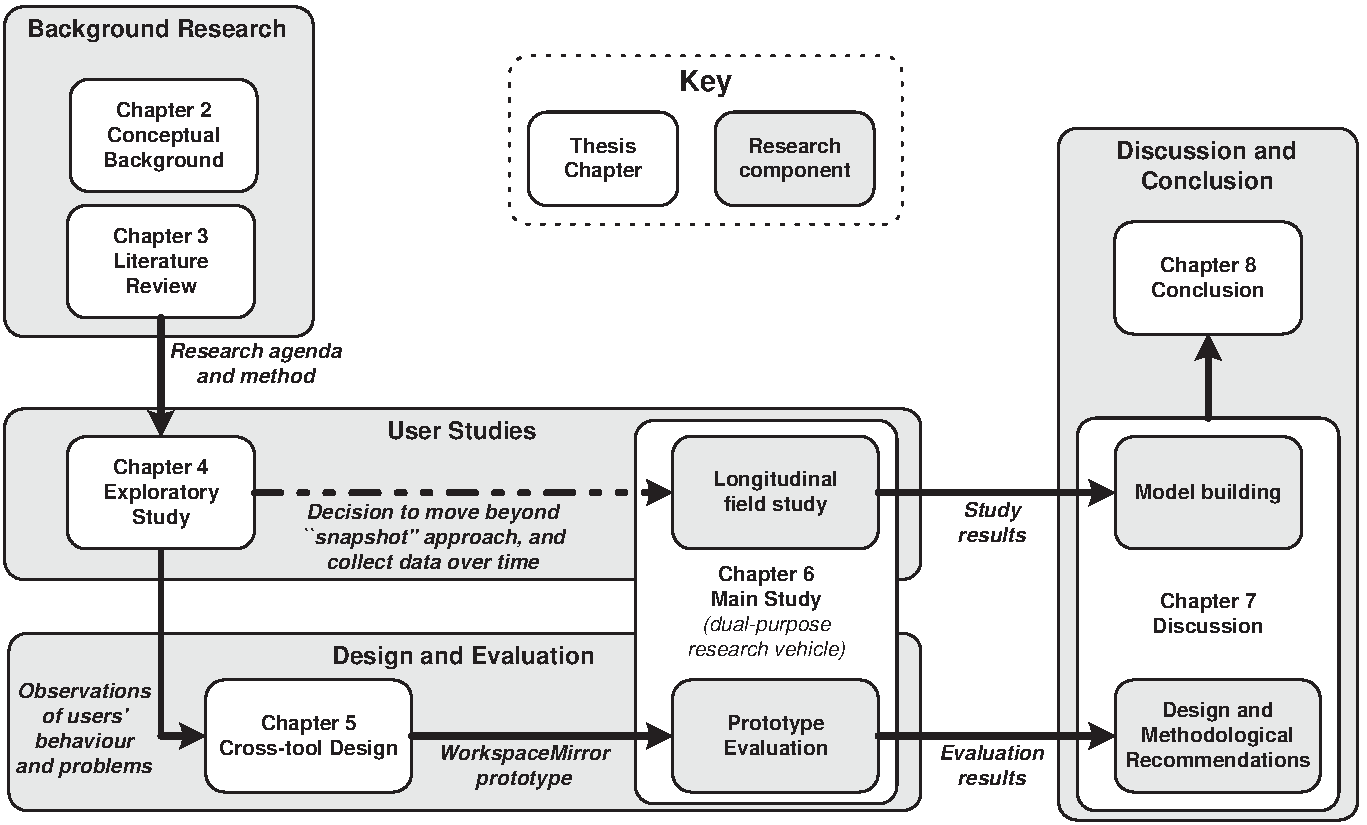
\includegraphics[width=1.0 \textwidth]{pictures/intro/Ch1-ThesisMap.pdf}
	\end{center}
	\caption{Overview of Thesis Structure} % \textit{Add contributions?}}
	\label{fig:intro:thesis_map}
\end{figure}

%%%%%%%%%%%%%%%
% Chapter 2: CF
%%%%%%%%%%%%%%%
% provides background for the thesis by reviewing related work within HCI and related disciplines. The chapter closes by discussing the initial aims which set the agenda for this research programme.
% details current support for PIM
% A conceptual framework relating to PIM. A descriptive vocabulary for discussing PIM as an activity, and the PIM-tools which enable it
% My Cross-tool Research Perspective/Analysis/Model of PIM. Provides theoretical framework for analysing user activity, user needs, discussing design, evaluation/study methodologies and results. Analysis of use of perspective.
% \item A high-level \textbf{conceptual framework} for PIM is proposed in \textbf{Chapter~\ref{chapter:bg}}. The framework defines terms used later in the thesis.  In particular a focus is taken on the integration of PIM-tools (\textit{substantive/minor}). 
% defines a number of concepts relevant to the thesis. 
% In this chapter, the author develops a \textit{conceptual framework} that 
\textbf{Chapter~\ref{chapter:bg}} provides an in-depth introduction to PIM.  Previous definitions of PIM are criticised, and a new view of PIM is developed in terms of four sub-activities performed with a collection of items: acquisition, organization, maintenance and retrieval.  Further conceptual background is provided relating to the current generation of commonly available PIM-tools. In particular, the concept of PIM-integration is defined and current integration mechanisms are surveyed.



%%%%%%%%%%%%%
% Chapter 3: REVIEW
%%%%%%%%%%%%%
% justification of techniques
% Critically assess
% \item A \textbf{critical review} of related research is presented in \textbf{Chapter~\ref{chapter:review}}. The review identifies a number of limitations of previous work, and motivates the research performed in the thesis (\textit{substantive/minor}).
\textbf{Chapter~\ref{chapter:review}} presents a \textit{critical analysis of previous research relevant to this thesis}.  Two main bodies of research are identified and surveyed: (1) empirical studies, and (2) prototype design.  Relevant theoretical work is also discussed. Limitations in prior research in the area of PIM-integration are used to motivate the thesis research agenda and methodology.  In particular, the limitations of previous technological research centred on radical invention are used to motivate the incremental design approach used in this thesis.

%%%%%%%%%%%%
% Chapter 4: EXP STUDY
%%%%%%%%%%%%
% \textit{Chapter 4 presents an exploratory study that compares how individuals manage their files, email and bookmarks. The potential for integrating these three tools is explored.}
% Add generation of scenarios?
% This chapter forms an empirical foundation for the rest of the thesis -- providing requirements and motivation for the design in \textbf{Chapter~\ref{chapter:design}}.  
\textbf{Chapter~\ref{chapter:exploratory_study}} reports an exploratory study aimed at comparing PIM behaviour across three collections of personal information -- document files, email and web bookmarks. The work can be contrasted with previous PIM studies which have focused on behaviour within one tool such as email. Key contributions include:
\begin{itemize}
%%%%%%%%%%%%%%%%%%%%%%%%
% EXP STUDY FINDINGS
%%%%%%%%%%%%%%%%%%%%%%%%
%  user requirements for improved integration between PIM tools
% Provide further understanding of PIM from a holistic "cross-tool" perspective. Use to differentiate.
% Probably want to break down in more detail!
% \item Further understanding of the nature of PIM in three specific tools (files, email and bookmarks), including new classifications of filing strategies in each tool, to reflect the observation of multiple strategies (\textit{substantive/minor}).
\item \textit{A comparison of PIM behaviour between files, email and bookmarks}  -- This analysis is centred on the four PIM sub-activities identified in \textbf{Chapter~\ref{chapter:bg}}.  % A particular focus is taken on the organizing sub-activity.

\item \textit{A new classification of organizing strategies in the file, email and bookmark contexts} -- Observations are made of \textit{multiple strategies} in each tool-specific context. Previous classifications of organizing strategies are criticized for not reflecting this  level of detail.  

% Third, a method for building a cross-tool profile of a user's management strategies.
% organizing strategies between tools for individual users.
\item \textit{A comparison of users' organizing strategies between files, email and bookmarks} -- Evidence is provided of variation in the extent of organizing performed by many participants across files, email and bookmarks.  A theoretical model is proposed to describe the multiple strategies observed both within and between collections.

% This major contribution encompasses three methodological contributions.
%%%%%%%%%%%%%%%%%%%%%
% ORG DIMENSION ANALYSIS
%%%%%%%%%%%%%%%%%%%%%
% First, a method for comparing folder structures in terms of their organizational dimensions on which folders are based.  
% analysing the organizational dimensions used to name folders in each tool context} --
\item \textit{A new technique for analysing the organizational dimensions used to name folders in each tool context} -- The most common types of folder are compared between the three tools.

%%%%%%%%%%%%%%%%%%%
% FOLDER OVERLAP ANALYSIS
%%%%%%%%%%%%%%%%%%%
% Second, a method for investigating the folder overlap between different PIM-tools for a particular user.  
\item \textit{A new technique for assessing the similarity of folder structures in two PIM-tools in terms of the number of folders they have in common} -- Significant folder overlap is highlighted for many participants, particularly between files and email.

%%%%%%%%%%%%%%%%%%%
% DESIGN RECOMMENDATIONS
%%%%%%%%%%%%%%%%%%%
\item \textit{A series of design implications for PIM-integration mechanisms} -- A number of PIM-related problems are identified which bridge multiple tool contexts, confirming the promise of improved integration between PIM-tools.  The above empirical findings suggest a number of potential routes for the design of such mechanisms.  In particular, the \textit{folder overlap} results provide the key empirical motivation for the design work in \textbf{Chapter~\ref{chapter:design}}.

\end{itemize}
% The study findings include the detailed analysis of similarities and differences between PIM practices across the three tools. 

%%%%%%%%%%%%%%%%%%%%%%%%%%%%%%%

%%%%%%%%%%%%%%%%%%%%%%%%%%%%%%%

%%%%%%%%%%%%%%%%%%%%%%%
% PART 2
% Chapter 5: DESIGN
%%%%%%%%%%%%%%%%%%%%%%%
% The second part of the thesis puts the developed cross-tool methodology into practice.
% \textit{Chapter 5 reports the design of WorkspaceMirror, motivated by the observation of folder overlap in Chapter 4.}
% The design is proposed as a research vehicle to: (1) explore the potential to improve integration between PIM tools, (2) develop appropriate methodology for evaluating PIM tools.  The chapter closes with an initial feasibility study to assess the potential of WorkspaceMirror.  Contributions from thesis are as follows:
% Cross-tool design of WorkspaceMirror and its implementation. Other designs? Why a useful contributions -- as design straw-man?
% \item The fourth main contribution, is the \textbf{design and implementation} of a prototype means of integration between PIM-tools, WorkspaceMirror, based on the folder-mirroring principle . The design is motivated by findings from the exploratory study (\textit{substantive/major}).  The notion of a cross-tool interactive artefact is also proposed (\textit{substantive/minor}).
\textbf{Chapter~\ref{chapter:design}} reports the cross-tool design and implementation work performed by the author.  In contrast to much previous design work in the area, the design approach is deliberately \textit{incremental} to facilitate user familiarity and systematic evaluation.  Contributions from the chapter are two-fold:
\begin{itemize}
% is informed by data from the exploratory study, WorkspaceMirror, a PIM-unification prototype designed and implemented by the candidate, is described.  
\item \textit{The design and implementation of WorkspaceMirror, a novel form of PIM-integration} -- The design is based on the principle of folder-mirroring, which allows the user to replicate the changes made in one folder structure to other PIM-tools.  A prototype is developed on the MS-Windows platform, offering folder-mirroring between the file, email and bookmark collections.  The design is motivated by the observations of \textit{folder overlap} in \textbf{Chapter~\ref{chapter:exploratory_study}}. 

\item \textit{Results from an initial evaluation of WorkspaceMirror} -- Positive feedback received from four of the five test users confirms the feasibility of the design.  The prototype is modified to accommodate participants' design suggestions.
\end{itemize}



%%%%%%%%%%%%%%%%%%%%%%%%
% Chapter 6: MAIN STUDY
%%%%%%%%%%%%%%%%%%%%%%%%
\textbf{Chapter~\ref{chapter:main-study}} reports a longitudinal field-study which acted as a dual-purpose research vehicle to: (1) evaluate the WorkspaceMirror prototype proposed in \textbf{Chapter~\ref{chapter:design}}, and (2) investigate PIM behaviour over time.  The investigation is differentiated from most previous studies in the area which have consisted of short-term ``snapshots'' of user behaviour.  A wide range of behaviour is reported through a series of case studies which highlight the idiosyncratic nature of PIM.  Two major sets of substantive contributions are offered: 
\begin{itemize}
%%%%%%%%%%%%%%%%%%%%%%%%%
% MAIN STUDY/EVALUATION
%%%%%%%%%%%%%%%%%%%%%%%%%
% Findings from combined Cross-tool Longitudinal Study/Formative Evaluation
%% A case-study evaluation (evaluation is hard to do
% Firstly, WorkspaceMirror is evaluated resulting in a number of proposed design improvements.
% aimed at investigating the impact of WorkspaceMirror on PIM practice. The evaluation involved eight users trialling WorkspaceMirror over a period of several months. The study also acted as a \textbf{longitudinal study} of PIM practice. In contrast most previous studies have consisted of ``snapshots'' of user behaviour.  
\item \textit{Results from the formative evaluation of WorkspaceMirror} -- The evaluation confirms the potential of mirroring top-level folders between PIM-tools, based on the positive feedback from many participants.  However, a trade-off is identified between the resulting consistency between folder structures, and users' needs for organizational flexibility in different tools.  A large number of design improvements are also suggested including the need for improved configurability.

%%%%%%%%%%%%%%%%%%%%%%%%%
% MAIN STUDY/STUDY
%%%%%%%%%%%%%%%%%%%%%%%%%
% \item Secondly, results from the longitudinal study of PIM over several months, including an analysis of changes in PIM strategy over time (\textit{substantive/major}). 
\item \textit{Insights into longitudinal PIM behaviour} -- Most study participants did not make major changes in organizing strategy.  Instead, \textit{incremental changes} were observed for two participants.  Balter's model of PIM strategies is criticised for not reflecting such subtle changes, and a new descriptive model is proposed.

The study findings also emphasise the background, supporting nature of PIM, and suggest that the participants devote little ongoing attention to PIM compared to their work tasks.  The study intervention causes increased reflection on PIM for many participants.  %  of findings are reported that suggest that participants rarely reflect on their PIM strategies. %, and instead are more focused on their work.

\end{itemize}
% \textit{Chapter 6 reports a field-study evaluation of WorkspaceMirror.}




%%%%%%%%%%%%%%
% Chapter 7: DISC
% WHERE IS THEPORY BUILDING?
%%%%%%%%%%%%%%
\textbf{Chapter~\ref{chapter:discussion}} discusses the substantive findings from the previous three chapters. The discussion offers four main contributions:
\begin{itemize}

% Extensions Barreau's PIM model~\citep{barreau:95} are proposed to encompass the supporting, ongoing, and cross-tool aspects of PIM, as identified in the empirical work in \textbf{Chapters~\ref{chapter:exploratory_study}}  and \textbf{~\ref{chapter:main-study}}. The chapter also considers implications for future work directed towards the design of more coherent, integrated PIM technologies.  The following contributions are offered:
% \item The main theoretical contribution is an extension of Barreau's PIM model~\citep{barreau:95} to encompass the ongoing, cross-tool supporting nature of PIM (\textit{substantive/major}). The model is based on empirical results from \textbf{Chapters~\ref{chapter:exploratory_study}} and\textbf{~\ref{chapter:main-study}}.
\item \textit{An extended conceptual framework of PIM} -- The view of PIM outlined in \textbf{Chapter~\ref{chapter:bg}} is extended to reflect the \textit{cross-tool}, \textit{supporting}, and \textit{ongoing} nature of PIM.  Each property is illustrated by reference to the empirical findings in earlier chapters.  The author offers the framework to outline potential routes for future theory development in the area.

%  The final substantive contribution is a set of recommendations for appropriate design routes for the design of mechanisms for improving integration between PIM-tools (\textit{substantive/major}).
\item \textit{A set of design implications for PIM-integration mechanisms} -- The evaluation results are discussed in the context of the extended framework.  Based on the experience of designing and evaluating WorkspaceMirror, the author argues that integration designs may offer strengths and weaknesses in different tool-specific and cross-tool contexts.  A number of design routes are highlighted for future integration work.

% Recommendations are made for appropriate methodology for evaluating PIM-tools based on experiences in evaluating WorkspaceMirror (\textit{methodological/minor}).
\item \textit{A set of methodological recommendations} -- The theoretical framework is used to structure a series of recommendations to guide the design and evaluation of PIM-integration mechanisms, derived from the experience of pursuing this research programme.  In particular, the dilemma of designing tools for supporting activities such as PIM is highlighted.

\item \textit{An exploration of potential evaluation metrics based on user experience} -- A number of participants in the main study reported in \textbf{Chapter~\ref{chapter:main-study}} were dissatisfied with their current organizing strategies and wanted to change them.  Such ``unsettledness'' is proposed as a indication of negative user experience in PIM.

\end{itemize}



%%%%%%%%%
% CONC
%%%%%%%%%
% before outlining potential future work. Chapter 8 presents overall conclusions, summarizes main contributions
% ties together
% bring together themes
% summarises
\textbf{Chapter~\ref{chapter:conclusion}} concludes the thesis by summarizing the main findings and contributions from the thesis.  Limitations of the research, and routes for further work are presented. % \footnote{\textit{This draft of Chapter 1 INTRODUCTION was printed \today}}.



%%%%%%%%%%%%%%%%%%%%%%%%%%%%%%%%%%%%
% Significance: major/minor (Weiss-Lijn)
% Audience: researchers/designers
% substantive and methodological
%%%%%%%%%%%%%%%%%%%%%%%%%%%%%%%%%%%%
% This thesis offers the following contributions. They are classified in terms of having a methodological or substantive nature, and their level of significance (major/minor):
% The section also considers their audience of interest (designers/researchers):%
% \begin{enumerate}

%%%%%%%%%%%%%%%%%%%%%%%%%%%%%%%%
% OTHER CONTRIBUTIONS TO CONSIDER
%%%%%%%%%%%%%%%%%%%%%%%%%%%%%%%%
% THINK: consideration of non-professional, social users?}
%%%%%%%%%%%%%%%%%%%%%%%%%%%%%%%%%%%%%%
% Methodological Contributions}
%%%%%%%%%%%%%%%%%%%%%%%%%%%%%%%%%%%%%% \textbf{M2: Methodological}. Operationalization as Cross-tool Methodology. Appraisal/analysis of use/validity of cross-tool method.

%%%%%%%%%%%%%%%%%%%%%%%%
% FIN: CONTRIBUTIONS
%%%%%%%%%%%%%%%%%%%%%%%%


%%%%%%%%%%%%%%%%%%%%%%%%%%%%%%
% Other possible challenges
%%%%%%%%%%%%%%%%%%%%%%%%%%%%%%
% Lots of commercial effort in terms of interface development.

%%%%%%%%%%%%%%%%%%%%%%%%%%%%%%%%%%%%%%%%%%%%%%%%%%%
\subsection{Publications relating to this Thesis}
%%%%%%%%%%%%%%%%%%%%%%%%%%%%%%%%%%%%%%%%%%%%%%%%%%%

The author has published a number of papers relating to this thesis work.  \citet{rpb:01b, rpb:01a} reports provisional results from the exploratory cross-tool study reported in \textbf{Chapter~\ref{chapter:exploratory_study}}. %, including the analysis of \textit{folder overlap}.

A subsequent series of papers report the design of WorkspaceMirror, along with the empirical results which motivated it~\citep{rpb:02b,rpb:02a,rpb:02c}. \citet{rpb:03a} adds preliminary results from the initial evaluation of WorkspaceMirror.

\citet{rpb:04a} presents a cross-section through the entire thesis, reporting aspects of the exploratory study, the design of WorkspaceMirror, and the longitudinal study. % presented in \textbf{Chapter~\ref{chapter:main-study}}.

Finally, \citet{rpb:04b}, outlines a Special Interest Group on PIM at the ACM CHI 2004 conference. The event has contributed to the establishment of a new PIM research community.  %  to 

